
% Inbuilt themes in beamer
\documentclass{beamer}

% Theme choice:
\usetheme{Warsaw}

% Title page details: 
\title{In the Shadow of a Giant: Medicare's Influence on Private Physician Payments} 
\subtitle{Jeffrey Clemens and Joshua D Gottlieb\\ \textit{Journal of Political Economy 2017}}
\author{Presented by: Ka Yan CHENG}
\date{ \vspace*{-1cm}\\ ECON 771 Health Economics II, Fall 2022}

% Fix the footline too long problem
\setbeamertemplate{headline}{}
\setbeamertemplate{footline}{%
  \leavevmode%
  \hbox{\begin{beamercolorbox}[wd=.5\paperwidth,ht=4.5ex,dp=2.125ex,leftskip=.3cm plus1fill,rightskip=.3cm]{author in head/foot}%
    \usebeamerfont{author in head/foot}\insertshortauthor
  \end{beamercolorbox}%
  \begin{beamercolorbox}[wd=.5\paperwidth,ht=4.5ex,dp=2.125ex,leftskip=.3cm,rightskip=.3cm plus1fil]{title in head/foot}%
    \usebeamerfont{title in head/foot}
    \parbox{.45\paperwidth}{\inserttitle}
  \end{beamercolorbox}}%
  \vskip0pt%
}

% Change subtitle format
\setbeamercolor{subtitle}{fg=lightgray}%
\setbeamerfont{subtitle}{size=\scriptsize}%



\setbeamerfont{date}{size=\footnotesize}


\begin{document}

% Title page frame
\begin{frame}
    \titlepage 
\end{frame}

% Remove logo from the next slides
\logo{}


% Outline frame
\begin{frame}{Outline}
    \tableofcontents
\end{frame}


% Lists frame
\section{Motivation}

\begin{frame}{Motivation}
\framesubtitle{In the Shadow of a Giant}
As a "giant" in the  market for physicians' services, we would expect payment rates set by Medicare, the federal insurer of the elderly and disabled, to influence private insurers' payments.\\
\hfill \break
It can be done through the following two channels:
\begin{enumerate}
\item Cost shifting (-ve)
\begin{itemize}
\item Reduction in Medicare's payment rates will be partially offset by private payment increases
\item Fixed cost
\item Discussion on it almost exclusively in the context of \textbf{hopsitals} (nonprofits' behavior in the presence of high fixed costs)
\item Theoretically less plausible in the context if \textbf{physician}'s practices
\end{itemize}
\item \textbf{Price following (+ve)} 
\begin{itemize}
\item Benchmarking
\item "the fee schedule in many contracts is stated as a percentage of the Medicare rate" (Gesme and Wiseman, 2010)
\end{itemize}
\end{enumerate}
\end{frame}

\begin{frame}{Motivation}
\framesubtitle{In the Shadow of a Giant -- Empirical evidence of Benchmarking to Medicare's payments}
\begin{center}
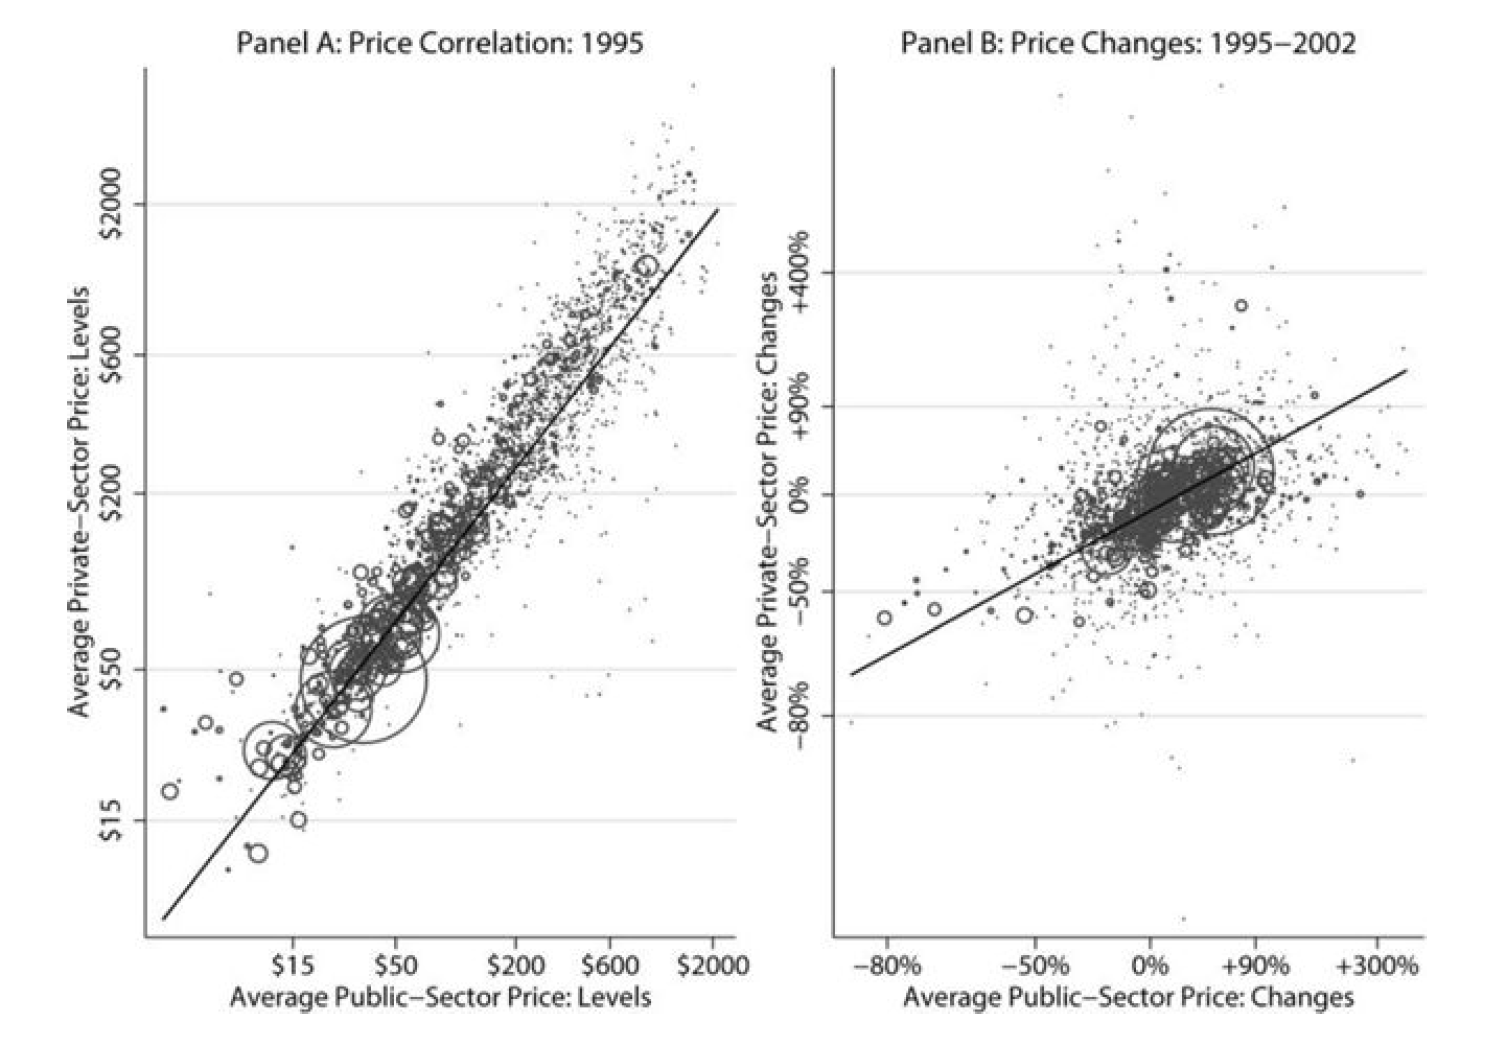
\includegraphics[height=6cm]{fig1}
\end{center}
Panel A: levels, Panel B: changes
\end{frame}

\begin{frame}{Motivation}
\framesubtitle{In the Shadow of a Giant -- Economic rationales of Benchmarking to Medicare's payments}
Economic rationales of Benchmarking to Medicare's payments:
\begin{enumerate}
\item Medicare will often be  relevant as a physician's outside option.
\item Medicare's relevant value scale contains a comprehensive accounting of treatement's relative input costs.\\
        (Updated estimates of physician's costs)
\item Help save the cost of negotiation between the insurer 
\end{enumerate}
\end{frame}

%Background
\section{Background}
\begin{frame}{Background}
\framesubtitle{Reimbursement from Medicare}
For service $j$, supplied in year $t$, by a provider in payment area $a$, the provider's reimbursement from Medicare  is approximately:
\begin{eqnarray*}
Reimbursement_{a,j,t} = Conversion Factor (CF)_{t,c(j)} \\
\times Relative Value Units (RAV)_{j,t} \\
\times Geographic Adjustment Factor (GAF)_{a,t}
\end{eqnarray*}
\end{frame}

\begin{frame}{Background}
\framesubtitle{2 Overhauls of  Medicare's Administrative Mechanism}
We need to overcome the concern that co-movement of price is simply due to productivity/demand shocks\\
\hfill \break
Historically, there is 2 overhauls of  Medicare's administrative mechanism that we can use:\\
\begin{enumerate}
\item Shock to Surgical versus Medical Payment 
\item Across-the-Board Payment Shocks
\end{enumerate}
\end{frame}

\begin{frame}{Background}
\framesubtitle{Shock to Surgical versus Medical Payment }
\begin{itemize}
\item In early 1990s: surgeons complained that slower growth in the use of their procedure should be rewarded
\item In 1993:  congress implemented the plan for the CMS to distinguish the CF for surgery and other services
\item Unequal payment spawned political discontent among nonsurgeons
\item Eliminated in 1998
\end{itemize}
\begin{center}
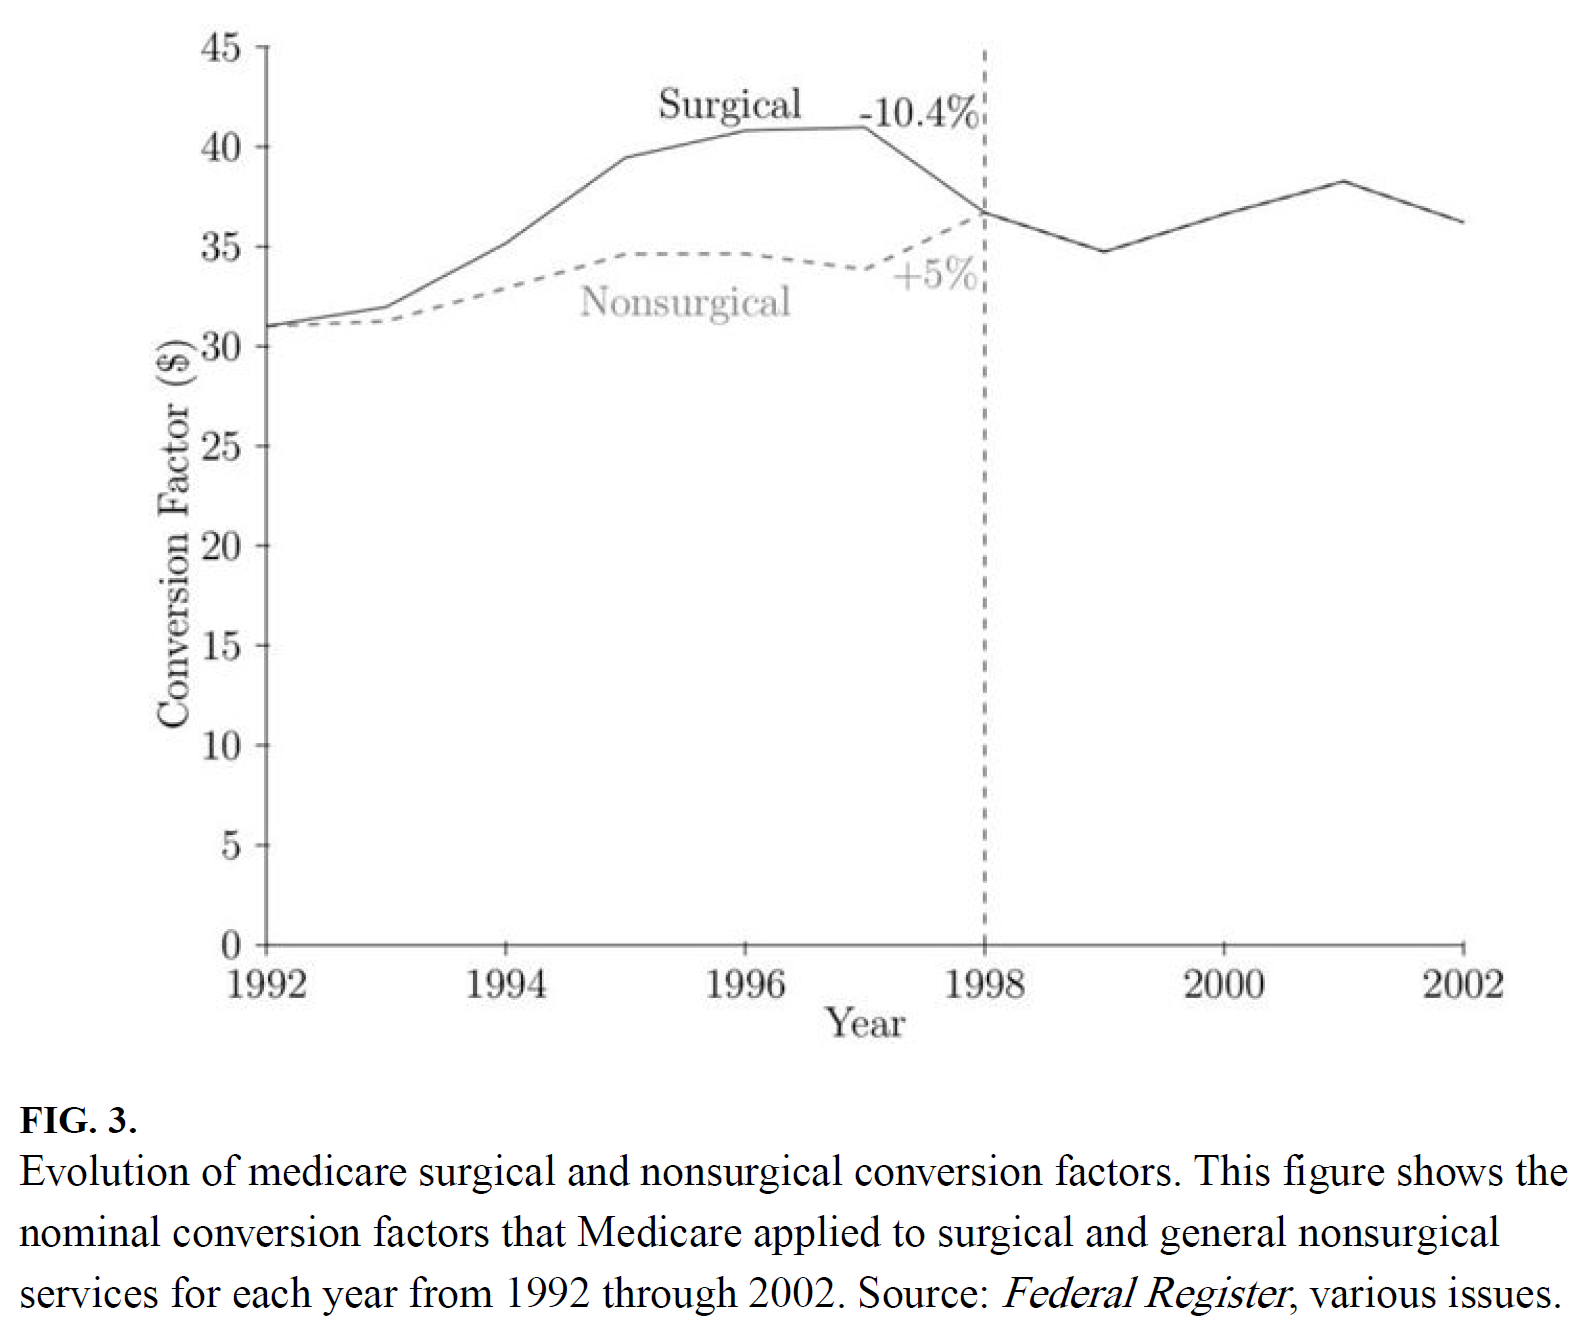
\includegraphics[height=4cm]{fig3}
\end{center}
\end{frame}

\begin{frame}{Background}
\framesubtitle{Across-the-Board Payment Shocks }
 $$Geographic Adjustment Factor (GAF)_{a,t}$$
\begin{itemize}
\item In 1997: the federal government consolidated 210 payment areas into 89 larger ones
\item These mergers were budget neutral within states
\item Reduced urban payments and enhanced rural payments

\end{itemize}
\end{frame}

%Reseach question
\section{Research questions}
\begin{frame}{Research questions}
\begin{enumerate}
\item \textbf{Medicare's influence on private insurers' payments for physician' services}
\item \textbf{How do the shock of the surgical conversion factor affect physician's behavior}
\item  Economic forces behind the influence 
\item  How can price following effect affect resouce allocation\\
(Physician Income and Specialty Choice)
\end{enumerate}
\end{frame}

%Contribution
\section{Contribution}
\begin{frame}{Contribution}
Show the indirect effects of Medicare's pricing decision
\begin{enumerate}
\item Overall price level in health sector
\item Physician's behavior
\end{enumerate}
\end{frame}

%Preview of findings
\section{Preview of findings}
\begin{frame}{Preview of findings}
\begin{enumerate}
\item \$1.00 increase in Medicare's payment increases private prices by more than one dollar
\item Regarding to the shock of the surgical conversion factor:
\begin{enumerate}
\item Surgeons reduced tehir proprnsity to accept new patients from both Medicare and private insurers
\item Sergeon become less likely to report being very satisfied with their career
\item less likely to pursue the continuing education needed to maintain board certification
\end{enumerate}
\end{enumerate}

\end{frame}

\section{Conceptual Framework}
\begin{frame}{Conceptual Framework}
\framesubtitle{Bargaining between one insurer and one physician group}
One insurer and one physician group negotiate on the reimbursement rate $r^*$ for the care that the group provides to the insurer's patients.\\
\hfill \break
The agreed payment rate:
$$r^* = (1-\theta)v_I + \theta u_{MD}$$
$\theta \in [0,1]$: Exogenous bargining weight of the insurer\\
$v_I$: Value of  \textbf{insurer}'s outside options (MC) \\
$u_{MD}$: Value of \textbf{physician}'s outside options (MB)\\
\hfill \break
If $\theta = 1$ (Full bargining power of the insurer), then $r^* = u_{MD}$\\
If $\theta = 0$ (No bargining power of the insurer ), then $r^* = v_I$
\end{frame}

\begin{frame}{Conceptual Framework}
\framesubtitle{Empirical Implications}
Consider 3 different scenarios, Physician has:
\begin{enumerate}
\item A constant MC and no capacity constraint \\
$\Rightarrow u_{MD} = c$\\
$\Rightarrow$ Outside option is saving the treatment cost\\
$\Rightarrow \frac{dr^*}{dr_M} = 0$
\hfill \break
\item Increasing MC\\
$\Rightarrow u_{MD} = f(r_M)$ with $f'(r_M)>0$\\
$\Rightarrow$ Altering MC of treating private patients\\
 $\Rightarrow \frac{dr^*}{dr_M} = \theta f'(r_M) >0$
\hfill \break
\item Operates at capacity\\
$\Rightarrow u_{MD} = ar_M$\\
$\Rightarrow$Revenue from treating $a$ Medicare patients instead \\
$\Rightarrow \frac{dr^*}{dr_M} =a \theta >0$
\end{enumerate}
\end{frame}

%Data
\section{Data}
\begin{frame}{Data}
\begin{enumerate}
\item Health care price data \\
	\begin{itemize}
	\item Medicare pricing
		\begin{itemize}
		\item Medicare claims from a 5\% random sample of the Part B (professional services and outpatient care) beneficiary population from 1995 to 2002
		\item Health Care Procedure Coding System (HCPCS) code for each service along with Medicare's payment
		\end{itemize}
	\item Private sector pricing
		\begin{itemize}
		\item Claim data from Thompson Reuters MarketScan database ("Med-Stat")
		\end{itemize}
	\end{itemize}
\item Measuring physician and insurer concentration
	\begin{itemize}
	\item Physician HHIs computed using group tax identifiers avaliable in the Medicare claims
	\end{itemize}
\item Physician welfare data from the community tracking study (CTS)
	\begin{itemize}
	\item Every two years, 12000 physicians in 60 geographic areas involved
	\item Four waves 1996-97, 1998-99, 2000-2001 and 2004-2005
	\end{itemize}
\end{enumerate}
\end{frame}

%Econometrics and identification
\section{Econometrics and identification}
\begin{frame}{Econometrics and identification}
\framesubtitle{Defining the shocks (as instruments to the medicare price change)}
\begin{enumerate}
\item Shock to Surgical versus Medical Payments
$$\text{PredChag}_j^{CF} =  \bar{P}_{j,pre}^{Medicare} \times (-0.104\text{Surgical}_j + 0.05\times \text{Nonsurgical}_j)$$
\hfill \break
\item Across-the-Board Payment Shocks
$$\text{PredChag}_a^{Geo} =   \bar{P}_{a,pre}^{Medicare} \times (GAF_A - GAF_a)$$
\end{enumerate}
\end{frame}

\begin{frame}{Econometrics and identification}
\framesubtitle{Estimation Framework for Price Responses}
Standard IV framework:
\begin{align*}
P^{Medicare}_{j.,a,t} = &  \pi \times \text{PredChg}_{j,a}^{Medicare} \times PostImplementation_{t} + X_{j,a,t}\phi_1 \\
& + \mu_j \mathbf{1}_j + \mu_a \mathbf{1}_a +  \mu_t \mathbf{1}_t + \mu_{j,a} \mathbf{1}_j\mathbf{1}_a + \mu_{t,s} \mathbf{1}_t\mathbf{1}_s + e_{j,a,t} \\
\end{align*}
$\pi$: how \$1 predicted Medicare change flows into Medicare payment of a service. Without measurement error, $\hat{\pi} = 1$.
\begin{align*}
P^{Private}_{j.,a,t} = &  \beta \times \widehat{\text{P}_{j,s,t}^{Medicare}} + X_{j,a,t}\phi_2 \\
& + \mu_j \mathbf{1}_j + \mu_a \mathbf{1}_a +  \mu_t \mathbf{1}_t + \mu_{j,a} \mathbf{1}_j\mathbf{1}_a + \mu_{t,s} \mathbf{1}_t\mathbf{1}_s + e_{j,a,t}
\end{align*}
\end{frame}

\begin{frame}{Results}
\framesubtitle{Estimation Framework for Price Responses}
\begin{center}
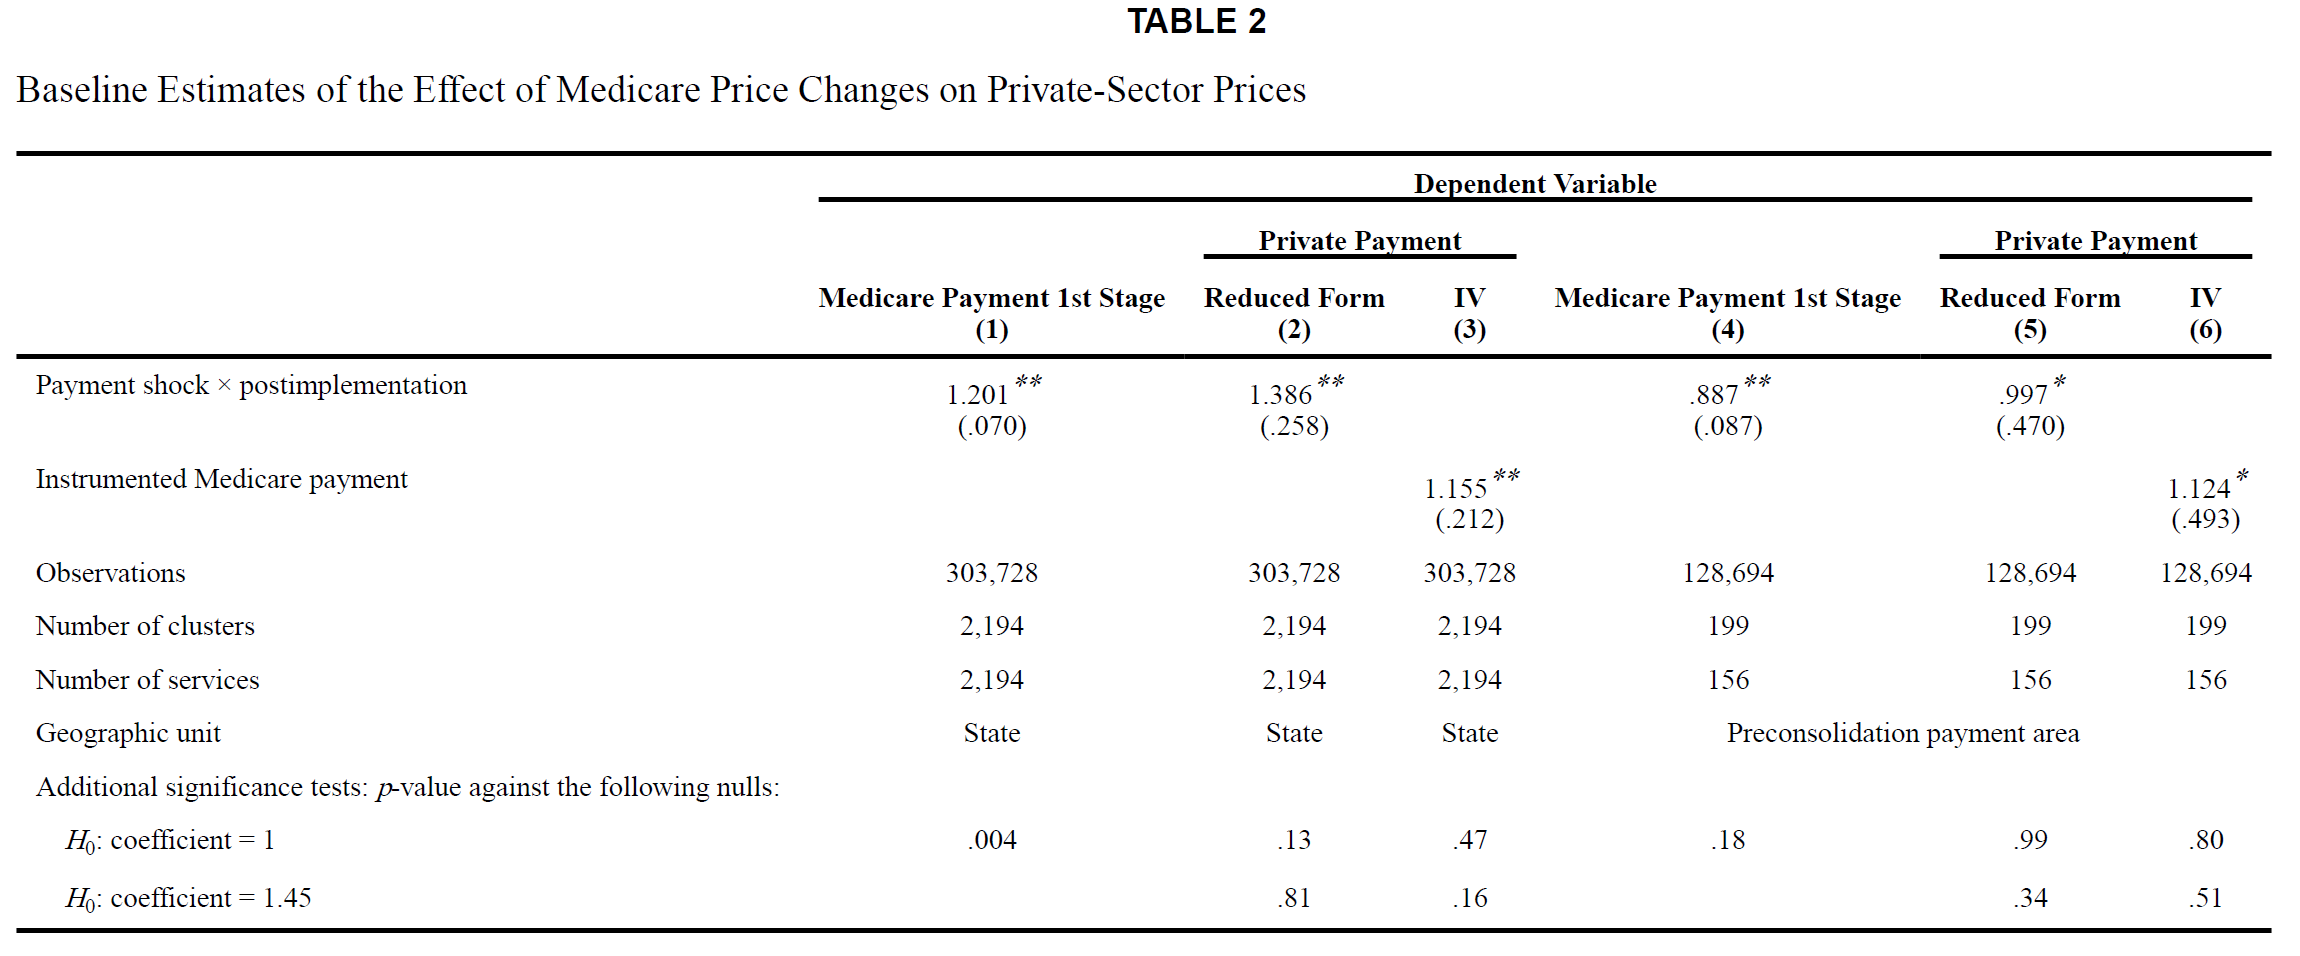
\includegraphics[height=4.5cm]{tab2}
\end{center}
Null hypothesis testing:
\begin{enumerate}
\item $\beta = 0$ (Fixed MC)
\item $\beta = 1$ (Insurer has full bargining power)
\item $\beta = 1.45$ (1.45: average scaling of private to Medicare payments, contract as ratio benchmarking)
\end{enumerate}
\end{frame}

\begin{frame}{Econometrics and identification}
\framesubtitle{Parametric Event Study}
Check the presnce of pre-existing trends in both Medicare and private payments
\begin{align*}
P^{Medicare}_{j.,a,t} = &  \sum_{t \neq t_0} \gamma_t \times \text{PredChg}_{j,a}^{Medicare}+ X_{j,a,t}\psi_{1} \\
& + \mu_j \mathbf{1}_j + \mu_a \mathbf{1}_a +  \mu_t \mathbf{1}_t + \mu_{j,a} \mathbf{1}_j\mathbf{1}_a + \mu_{t,s} \mathbf{1}_t\mathbf{1}_s + u_{j,a,t} \\
\end{align*}
\begin{align*}
P^{Private}_{j.,a,t} = &  \sum_{t \neq t_0} \delta_t \times \text{PredChg}_{j,a}^{Medicare}+ X_{j,a,t}\psi_{2} \\
& + \mu_j \mathbf{1}_j + \mu_a \mathbf{1}_a +  \mu_t \mathbf{1}_t + \mu_{j,a} \mathbf{1}_j\mathbf{1}_a + \mu_{t,s} \mathbf{1}_t\mathbf{1}_s + v_{j,a,t}
\end{align*}
\end{frame}

%Results
\section{Results}
\begin{frame}{Results}
\framesubtitle{Parametric Event Study - Elimination of the surgical conversion factor}
\begin{center}
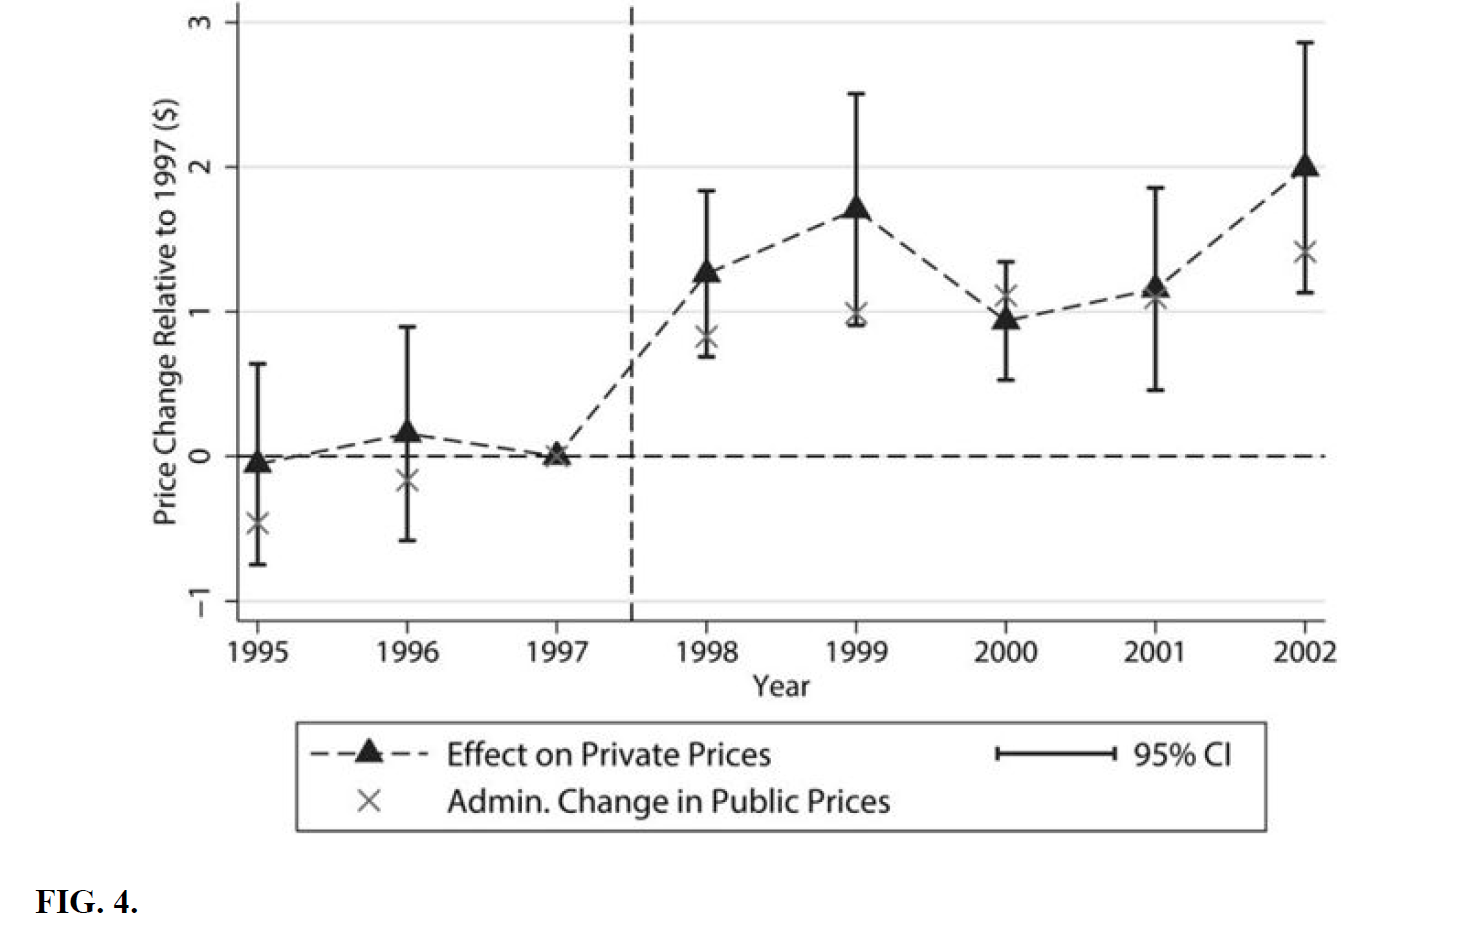
\includegraphics[height=7cm]{fig4}
\end{center}
\end{frame}

\begin{frame}{Results}
\framesubtitle{Parametric Event Study - Geographical payment shocks}
\begin{center}
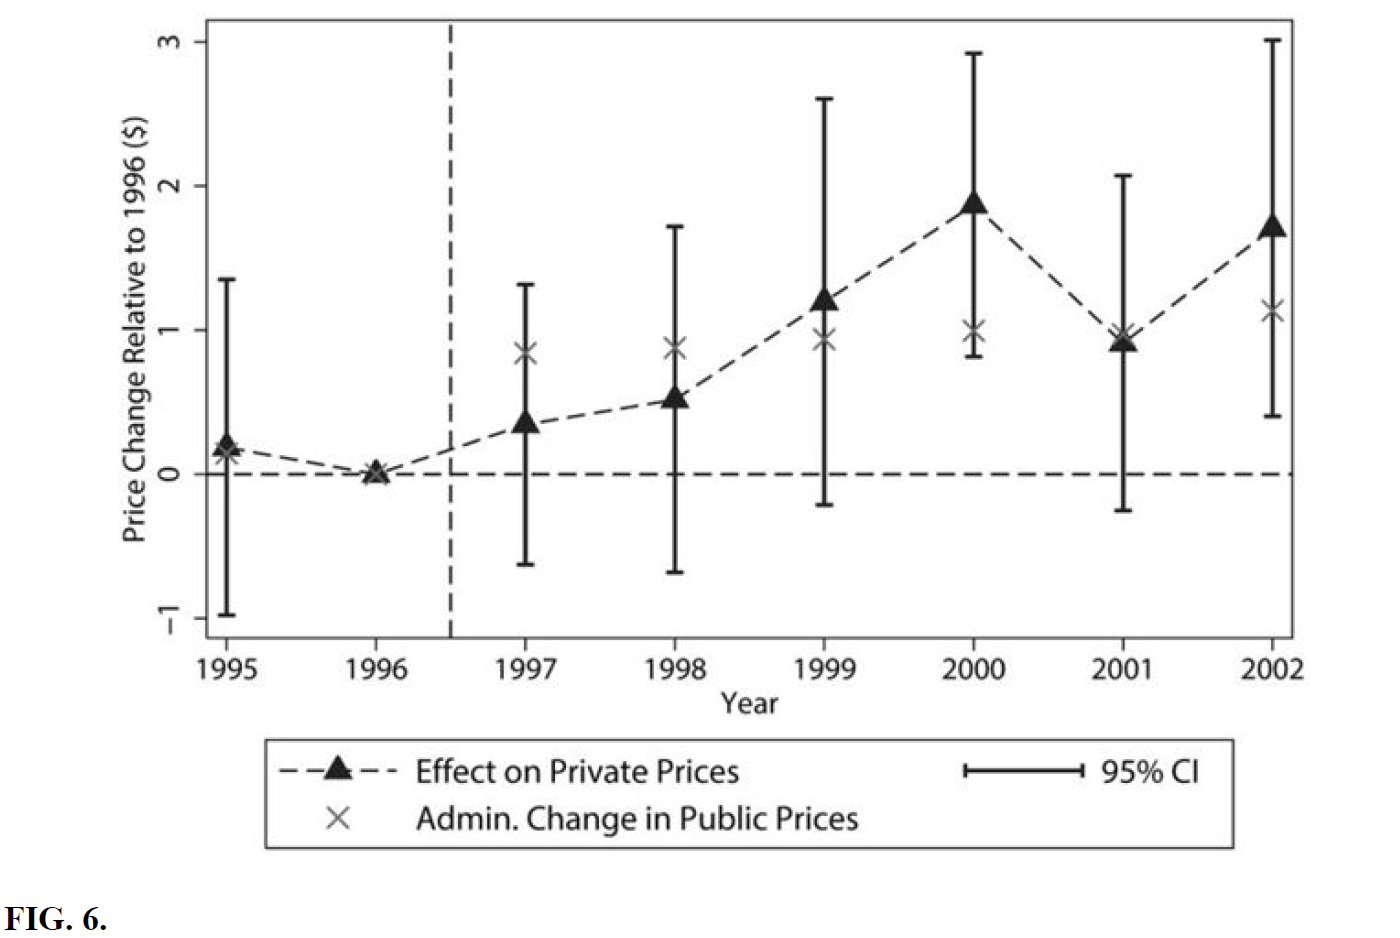
\includegraphics[height=7cm]{fig6}
\end{center}
\end{frame}

\begin{frame}{Econometrics and identification}
\framesubtitle{Estimation Framework for Physician Outcomes}
Standard DID framework
\begin{align*}
y_{it} = & \kappa \text{Surgeon}_i \times \text{PostImplemetation}_t \\
& + \lambda Surgeon_i + \chi_t \text{SurveyWave}_t + \varepsilon_{it}
\end{align*}
$y_{it}$: \\
\begin{enumerate}
\item work hours
\item propensity to take new patients
\item career satisfaction
\item maintenance of board certification evolved for surgeons relative to other physicians
\end{enumerate}
\end{frame}

\begin{frame}{Results}
\framesubtitle{Estimation Framework for Physician Outcomes}
\begin{center}
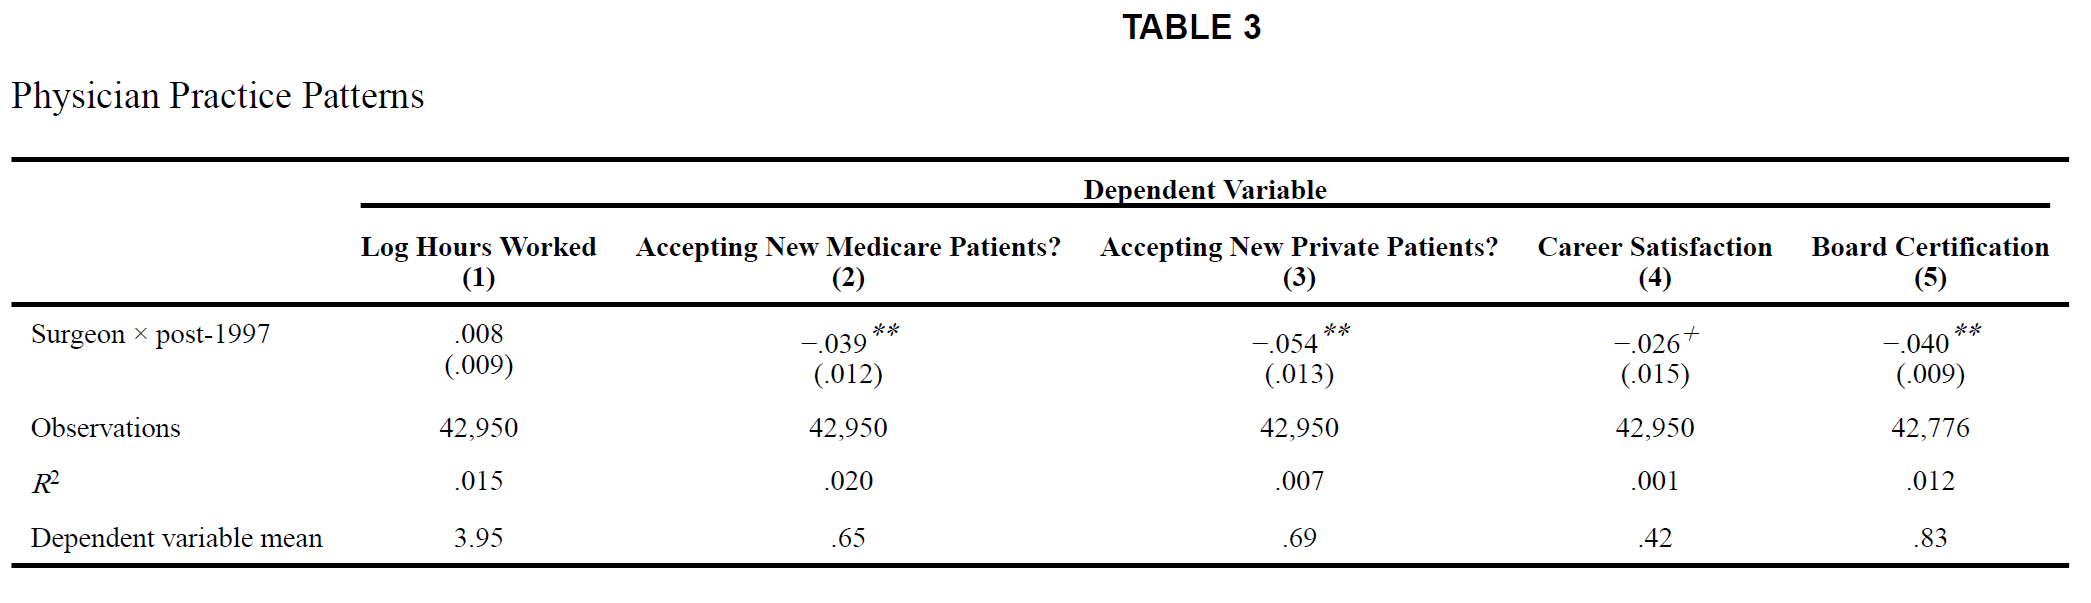
\includegraphics[height=3.25cm]{tab3}
\end{center}
\end{frame}

%Threats
\section{Threats/Discussions}
\begin{frame}{Threats/Discussions}
Is cost shifting really not likely to happen in the context of physicians' practices?
\end{frame}

%Results
\section{Conclusion}
\begin{frame}{Conclusion}
Due to the price following effect, Medicare's pricing decision can induce overall inflation in the health market, which also affects physician's behaviors and the real allocation of the society.

\end{frame}

\end{document}